\section{System STLC-Impure}

This chapter describes an extension of the system STLC-Pure with free
functions. As there's a subtyping relation between stoic functions and
free functions, it's natural to integrate subtyping in the system.

We'll first introduce the formalization, then discuss soundness and
effect safety. In the discussion, we'll focus on its difference from
the system STLC-Pure.

\subsection{Definitions}

Initially, we arrived at a formulation of the system shown in
Figure~\ref{fig:stlc-impure-definition-first}. It's a straight-forward
extension of STLC-Pure with subtyping and free functions.

The definition is all good, except that preservation breaks. The
problem is caused by using an impure term as \emph{Top}. To see a
concrete example, let's assume $\Gamma = \{c:E\}$. It's obvious that
following typing relation holds:

\begin{center}
  $\{c:E\} \vdash (\lambda x:Top. \; \lambda y:B. \; x) \; c \; : \; B \to Top$
\end{center}

However, after one evaluation step\footnote{Note that variables are
  values, thus we can take a step here. We can also construct a
  counter-example by wrap $c$ in a free function like
  $\lambda x:B. c$.}, we get the term $\lambda y:B. \; c$, which can
at best be typed as $B \Rightarrow Top$. Thus preservation
breaks. This problem leads us to two different formulations.

\begin{figure}
\begin{framed}

% multi-column separator
\setlength{\columnseprule}{0.4pt}
\begin{multicols}{2}

\textbf{Syntax}

\begin{tabu} to \linewidth {l l l X[r]}
  t   & ::= &                    & terms:               \\
      &     &  x                 & variable             \\
      &     & $\lambda$ x:T.t    & abstraction          \\
      &     & t t                & application          \\
\\
  v   & ::= &                    & values:              \\
      &     & $\lambda$ x:T.t    & abstraction value    \\
      &     & x                  & variable value       \\
\\
  T   & ::= &                    & types:               \\
      &     & \colorbox{shade}{Top}  & top type             \\
      &     & B                  & basic type           \\
      &     & E                  & capability type      \\
      &     & T $\to$ T          & type of stoic funs       \\
      &     & \colorbox{shade}{T $\Rightarrow$ T} & type of free funs   \\
\end{tabu}

\hfill\\

\textbf{Evaluation} \hfill \framebox[1.2\width][r]{$t \longrightarrow t'$}

\infrule[E-App1]
{ t_1 \longrightarrow t'_1 }
{ t_1 \; t_2 \longrightarrow t'_1 \; t_2 }

\infrule[E-App2]
{ t_2 \longrightarrow t'_2 }
{ v_1 \; t_2 \longrightarrow v_1 \; t'_2 }

\infax[E-AppAbs]
{ (\lambda x:T.t_1) v_2 \longrightarrow [x \mapsto v_2]t_1 }

\textbf{Pure Environment}

\hfill

\begin{center}
\begin{tabular}{l c l}
pure($\varnothing$)                   & = &   $\varnothing$ \\
pure($\Gamma$, x: E)                  & = &  pure($\Gamma$) \\
\rowcolor{gray!40}
pure($\Gamma$, x: S $\Rightarrow$ T)  & = &  pure($\Gamma$) \\
pure($\Gamma$, x: T)                  & = &  pure($\Gamma$), x: T     \\
\end{tabular}
\end{center}

\columnbreak

\textbf{Typing}  \hfill \framebox[1.2\width][r]{$\Gamma \vdash x : T$}

\infrule[T-Var]
{ x: T \in \Gamma }
{ \Gamma \vdash x : T }

\infrule[T-Abs1]
{ pure(\Gamma),\; x: S \vdash t_2 : T }
{ \Gamma \vdash \lambda x:S.t_2 : S \to T }

\infrule[T-Abs2]
{  \colorbox{shade}{$\Gamma,\; x: S \vdash t_2 : T$} }
{  \colorbox{shade}{$\Gamma \vdash \lambda x:S.t_2 : S \Rightarrow T$} }

\infrule[T-App]
{ \Gamma \vdash t_1 : S \to T \andalso \Gamma \vdash t_2 : S }
{ \Gamma \vdash t_1 \; t_2 : T }

\infrule[T-Sub]
{  \colorbox{shade}{$\Gamma \vdash t : S \andalso S <: T$} }
{  \colorbox{shade}{$\Gamma \vdash t : T$} }

\colorbox{shade}{\textbf{Subtyping}}  \hfill \framebox[1.2\width][r]{$S <: T$}

\infax[S-Top]{ T <: Top }

\infax[S-Refl]{ T <: T }

\infrule[S-Trans]
{ S <: U \andalso U <: T }
{ S <: T }

\infax[S-Degen]
{ S \to T <: S \Rightarrow T }

\infrule[S-Fun1]
{ S1 <: S2 \andalso T2 <: T1 }
{ S2 \to T2 <: S1 \to T1 }

\infrule[S-Fun2]
{ S1 <: S2 \andalso T2 <: T1 }
{ S2 \Rightarrow T2 <: S1 \Rightarrow T1 }

\hfill\\

\end{multicols}
\end{framed}

\caption{System STLC-Impure First Formulation}
\label{fig:stlc-impure-definition-first}
\end{figure}

The first one is to introduce two different Top types, one is pure and
the other is impure\footnote{This idea is suggested by Sandro
  Stucki.}. The capability type E and free function type
$S \Rightarrow T$ are not subtypes of the pure Top. The subtyping
hierarchy is shown in
Figure~\ref{fig:stlc-impure-subtyping-tree}. This formulation works
well, and we've proved soundness and effect safety for the
formulation. However, we lose the simplicity of the type system. And
it's counter-intuitive to forbid Top in pure environments, as we
cannot create side effects with a variable of the type Top.

\begin{figure}
\centering

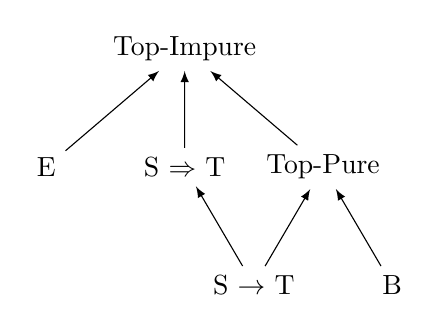
\begin{tikzpicture}[sibling distance=5em,
  every node/.style = {align=center},
  edge from parent/.style={draw,latex-}]
  \node {Top-Impure}
  child { node {E} }
  child { node (free) {S $\Rightarrow$ T} }
  child { node {Top-Pure}
    child { node (stoic) {S $\to$ T} }
    child { node {B} } };
  \path [draw, -latex] (stoic) -- (free);
\end{tikzpicture}

\caption{Subtyping: Top-Pure and Top-Impure}
\label{fig:stlc-impure-subtyping-tree}
\end{figure}

The second possibility is to keep the elegance of the type system and
change the evaluation rules. All terms of the type Top are equivalent,
because we can do nothing with a term of the type Top. This
observation inspires us to introduce a \emph{top} value and replace
the standard \textsc{E-AppAbs} rule with two evaluation rules as
follows:

\begin{multicols}{2}

\infrule[E-AppAbs1]
{ T \neq Top }
{ (\lambda x:T.t_1) v_2 \longrightarrow [x \mapsto v_2]t_1 }

\infrule[E-AppAbs2]
{ T = Top }
{ (\lambda x:T.t_1) v_2 \longrightarrow [x \mapsto top]t_1 }

\end{multicols}

The two rules have the effect that if a function takes a parameter of
the type Top, when called it will drop the passed parameter and
replace it with the value \emph{top}. We follow this approach in the
formulation and the full definition is presented in
Figure~\ref{fig:stlc-impure-definition}.

\begin{figure}
\begin{framed}

% multi-column separator
\setlength{\columnseprule}{0.4pt}
\begin{multicols}{2}

\textbf{Syntax}

\begin{tabu} to \linewidth {l l l X[r]}
  t   & ::= &                    & terms:               \\
      &     & \colorbox{shade}{top} & top value            \\
      &     & x                  & variable             \\
      &     & $\lambda$ x:T.t    & abstraction          \\
      &     & t t                & application          \\
\\
  v   & ::= &                    & values:              \\
      &     & $\lambda$ x:T.t    & abstraction value    \\
      &     & x                  & variable value       \\
      &     & \colorbox{shade}{top}  & top value            \\
\\
  T   & ::= &                    & types:               \\
      &     & \colorbox{shade}{Top}  & top type             \\
      &     & B                  & basic type           \\
      &     & E                  & capability type      \\
      &     & T $\to$ T          & type of stoic funs       \\
      &     & \colorbox{shade}{T $\Rightarrow$ T} & type of free funs   \\
\end{tabu}

% \hfill\\
\vspace{0.1em}

\textbf{Evaluation} \hfill \framebox[1.2\width][r]{$t \longrightarrow t'$}

\infrule[E-App1]
{ t_1 \longrightarrow t'_1 }
{ t_1 \; t_2 \longrightarrow t'_1 \; t_2 }

\infrule[E-App2]
{ t_2 \longrightarrow t'_2 }
{ v_1 \; t_2 \longrightarrow v_1 \; t'_2 }

\infrule[E-AppAbs1]
{ \colorbox{shade}{$T \neq Top$} }
{ \colorbox{shade}{$(\lambda x:T.t_1) \; v_2 \longrightarrow [x \mapsto v_2]t_1$} }

\infrule[E-AppAbs2]
{ \colorbox{shade}{$T = Top$} }
{ \colorbox{shade}{$(\lambda x:T.t_1) \; v_2 \longrightarrow [x \mapsto top]t_1$} }

\textbf{Pure Environment}

\hfill

\begin{center}
\begin{tabular}{l c l}
pure($\varnothing$)                   & = &   $\varnothing$ \\
pure($\Gamma$, x: E)                  & = &  pure($\Gamma$) \\
\rowcolor{gray!40}
pure($\Gamma$, x: S $\Rightarrow$ T)  & = &  pure($\Gamma$) \\
pure($\Gamma$, x: T)                  & = &  pure($\Gamma$), x: T     \\
\end{tabular}
\end{center}

\columnbreak

\textbf{Typing}  \hfill \framebox[1.2\width][r]{$\Gamma \vdash x : T$}

\infax[T-Top]{ \colorbox{shade}{$\Gamma \vdash top : Top$} }

\infrule[T-Var]
{ x: T \in \Gamma }
{ \Gamma \vdash x : T }

\infrule[T-Abs1]
{ pure(\Gamma),\; x: S \vdash t_2 : T }
{ \Gamma \vdash \lambda x:S.t_2 : S \to T }

\infrule[T-Abs2]
{  \colorbox{shade}{$\Gamma,\; x: S \vdash t_2 : T$} }
{  \colorbox{shade}{$\Gamma \vdash \lambda x:S.t_2 : S \Rightarrow T$} }

\infrule[T-App]
{ \Gamma \vdash t_1 : S \to T \andalso \Gamma \vdash t_2 : S }
{ \Gamma \vdash t_1 \; t_2 : T }

\infrule[T-Sub]
{  \colorbox{shade}{$\Gamma \vdash t : S \andalso S <: T$} }
{  \colorbox{shade}{$\Gamma \vdash t : T$} }

\colorbox{shade}{\textbf{Subtyping}}  \hfill \framebox[1.2\width][r]{$S <: T$}

\infax[S-Top]{ T <: Top }

\infax[S-Refl]{ T <: T }

\infrule[S-Trans]
{ S <: U \andalso U <: T }
{ S <: T }

\infax[S-Degen]
{ S \to T <: S \Rightarrow T }

\infrule[S-Fun1]
{ S1 <: S2 \andalso T2 <: T1 }
{ S2 \to T2 <: S1 \to T1 }

\infrule[S-Fun2]
{ S1 <: S2 \andalso T2 <: T1 }
{ S2 \Rightarrow T2 <: S1 \Rightarrow T1 }

\hfill\\

\end{multicols}
\end{framed}

\caption{System STLC-Impure}
\label{fig:stlc-impure-definition}
\end{figure}

Note that in current system, we need to change the definition of the
function \emph{pure} to exclude free function types from the pure
environment. This restriction is important, because there's no way to
know what side effects there might be inside free functions. If stoic
functions have access to free functions, we'll loose the ability to
track the effects of stoic functions in the type system.

In principle, we can keep some free functions that can never be called
in the pure environment, such as $(B \to E) \Rightarrow B$, as it's
impossible to get an actual instance of the inhabitable type $B \to E$
in order to call this function. However, it's not useful to have
functions in the environment if they can never be called. Thus, to
simplify the system without sacrificing usability, we removed all free
function types from the pure environment.

\subsection{Soundness}

We proved both progress and preservation of the system.

\begin{theorem}[Progress]
If $\varnothing \vdash t : T$, then either $t$ is a value or there is some
$t'$ with $t \longrightarrow t'$.
\end{theorem}

\begin{theorem}[Preservation]
If $\Gamma \vdash t : T$, and $t \longrightarrow t'$, then $\Gamma
\vdash t' : T$.
\end{theorem}

As you can imagine, now we need two different substitution lemmas in
the proof of preservation, corresponding to the two reduction rules.

\begin{lemma}[Subsitution-Not-Top]
  If $\Gamma,\; x:S \vdash t : T$, $S \neq Top$, s is a value and
  $\Gamma \vdash s : S$, then $\Gamma \vdash [x \mapsto s]t : T$.
\end{lemma}

\begin{lemma}[Subsitution-Top]
  If $\Gamma,\; x:Top \vdash t : T$, then $\Gamma \vdash [x \mapsto top]t : T$.
\end{lemma}

We restrict $s$ to be a value in the lemma \emph{Substitution-Not-Top}
for the same reason as in the system STLC-Pure.

\subsection{Effect Safety}

We follow the same approach as in the system STLC-Pure in the
formulation of effect safety. The formulation is an extension of the
definition of \emph{capsafe} and \emph{caprod} in STLC-Pure with free
function types.

\subsubsection{Formulation}

The definitions of \emph{inhabitable types} and \emph{inhabitable
  environment} are the same as in the system STLC-Pure.

With the presence of free functions, the previous formulation of
effect safety is not enough. We not only need to ensure that it's
impossible to construct a term of the capability type in pure and
inhabitable environments, but also need to ensure only stoic functions
can be called in pure and inhabitable environments. The two conditions
together guarantee that there cannot be actual side effects inside a
pure stoic function. Thus, we need two statements about effect safety.

\begin{definition}[Effect-Safety-Inhabitability-1]
  If $\Gamma$ is a pure and inhabitable environment, then there
  doesn't exist $t$ with $\Gamma \vdash t : E$.
\end{definition}

\begin{definition}[Effect-Safety-Inhabitability-2]
  If $\Gamma$ is a pure and inhabitable environment, and
  $\Gamma \vdash t_1 \; t_2 : T$, then there exists U, V such that
  $\Gamma \vdash t_1 : U \to V$.
\end{definition}

A tempting formulation of the second effect safety statement would be
that \emph{in a pure and inhabitable environment it's impossible to
  construct a term of the free function type}. However, this
formulation has no hope to be proved, as $S \to T$ is a subtype of
$S \Rightarrow T$, any term that can be typed as the former can also
be typed as the latter.

As in the system STLC-Pure, the proof of these two statements depends
on two weaker and more general statements about \emph{healthy
  environments}. If we can arrive at such a definition of
\emph{healthy environment} that a pure and inhabitable environment is
also healthy, then it suffices to prove following two statements about
healthy environments:

\begin{definition}[Effect-Safety-1]
  If $\Gamma$ is healthy, there doesn't exist $t$ with
  $\Gamma \vdash t : E$.
\end{definition}

\begin{definition}[Effect-Safety-2]
  If $\Gamma$ is healthy and $\Gamma \vdash t_1 \; t_2 : T$, then
  there exists U, V such that $\Gamma \vdash t_1 : U \to V$.
\end{definition}

Now we need to extend the definition of \emph{capsafe} and
\emph{caprod} for free function types. Our first attempt is to add
following rule:

\infax[CP-Fun2]{ S \Rightarrow T \quad caprod }

With this rule, the type $(B \Rightarrow B) \to E$ would be considered
\emph{capsafe}, according to the rule \textsc{CS-Fun1}. However, with
a variable $f$ of this type and another variable $g$ of the
\emph{capsafe} type $B \to B$ in the healthy environment, the
constructed term \emph{f g} has the capability type E; the first
statement of effect safety breaks. This formulation also breaks the
connection between pure inhabitable environments and healthy
environments. A pure and inhabitable environment is no longer
healthy. For example, the type $B \to B \Rightarrow B$ is pure and
inhabitable, but it's not \emph{capsafe}.

On the other hand, we cannot do the opposite to take $S \Rightarrow T$
as \emph{capsafe}, as it would allow calling free functions in healthy
environments; the second statement of effect safety breaks. In the
meanwhile, the pure and inhabitable type $(B \Rightarrow E) \to E$ is
not \emph{capsafe}, thus a pure and inhabitable environment is no
longer a healthy environment.

This dilemma prompts us to reexamine the meaning of \emph{capsafe} and
\emph{caprod}. When these facilities were first introduced in
STLC-Pure, they were formulated in terms of the provability of the
capability type E. From the perspective of the provability of E,
$S \to T$ and $S \Rightarrow T$ don't make much difference. Thus, free
function types should be formulated the same way as stoic function
types. We tried this approach, and it worked\footnote{Sandro Stucki
  suggested to take this approach.}. The full formulation is presented
in Figure~\ref{fig:stlc-impure-healthy-definition}.

\begin{figure}[h]
\begin{framed}

% multi-column separator
\setlength{\columnseprule}{0.4pt}
\begin{multicols}{2}

\textbf{Capsafe}

\infax[CS-Base]
{ B \quad \text{capsafe} }

\infrule[CS-Fun1]
{ S \quad caprod }
{ S \to T \quad \text{capsafe} }

\infrule[CS-Fun2]
{ T \quad \text{capsafe} }
{ S \to T \quad \text{capsafe} }

\infrule[CS-Fun3]
{ \colorbox{shade}{$S \quad caprod$} }
{ \colorbox{shade}{$S \Rightarrow T \quad \text{capsafe}$} }

\infrule[CS-Fun4]
{ \colorbox{shade}{$T \quad \text{capsafe}$} }
{ \colorbox{shade}{$S \Rightarrow T \quad \text{capsafe}$} }

\columnbreak

\textbf{Caprod}

\infax[CP-Eff]
{ E \quad caprod }

\infrule[CP-Fun1]
{ S \; \text{capsafe} \andalso T \; caprod }
{ S \to T \quad caprod }

\infrule[CP-Fun2]
{ \colorbox{shade}{$S \; \text{capsafe} \andalso T \; caprod$} }
{ \colorbox{shade}{$S \Rightarrow T \quad caprod$} }

\textbf{Healthy}

\infax[H-Empty]
{ \varnothing \quad caprod }

\infrule[H-Var]
{ G \; healthy \andalso T \; \text{capsafe} }
{ G, \; x:T \quad healthy }

\hfill\\

\end{multicols}
\end{framed}

\caption{System STLC-Impure Healthy Environment}
\label{fig:stlc-impure-healthy-definition}
\end{figure}

Now a healthy environment is no longer pure. For example, the type
$B \Rightarrow B$ is \emph{capsafe}, but it's not pure. As a
consequence, we need to slightly update the definition of the second
statement of effect safety:

\begin{definition}[Effect-Safety-2']
  If $\Gamma$ is pure and healthy, and $\Gamma \vdash t_1 \; t_2 : T$,
  then there exists U, V such that $\Gamma \vdash t_1 : U \to V$.
\end{definition}

Why this formulation of healthy environment is acceptable? In short,
it's because the statement \emph{Effect-Safety-1} and
\emph{Effect-Safety-2'} logically imply the statement
\emph{Effect-Safety-Inhabitability-1} and
\emph{Effect-Safety-Inhabitability-2} respectively.

The logical implications hold because a pure and inhabitable
environment is also a healthy (and pure) environment. This claim has
been formally proved:

\begin{lemma}[Inhabitable-Capsafe]
  If the type T is inhabitable, then either T is capsafe or $T = E$ or
  T is a free function type.
\end{lemma}

\begin{theorem}[Inhabitable-Pure-Healthy]
  If $\Gamma$ is pure and inhabitable, then $\Gamma$ is healthy.
\end{theorem}

\begin{theorem}[Inhabitable-Pure-Healthy']
  If $\Gamma$ is pure and inhabitable, then $\Gamma$ is pure and
  healthy.
\end{theorem}

Note that the last theorem follows immediately from the second one, as
we already know from the premise that $\Gamma$ is pure.

% From the theorems above, it's obvious that any property proved for a
% healthy (and pure) environment also holds for a pure and inhabitable
% environment. Therefore, it suffices to prove the statement
% \emph{Effect-Safety-1} and \emph{Effect-Safety-2'}.

\subsubsection{Proof}

The proof of the first statement of effect safety is almost the same
as in STLC-Pure. The only change worth mention is that, in the
presence of subtyping, an additional lemma \emph{Capsafe-Sub} is
required.  The first effect safety statement follows immediately from
the lemma \emph{Healthy-Capsafe}.

\begin{lemma}[Capsafe-Not-Caprod]
 If type T is capsafe, then T is not caprod.
\end{lemma}

\begin{lemma}[Capsafe-Or-Caprod]
 For any T, T is either capsafe or caprod.
\end{lemma}

\begin{lemma}[Capsafe-Sub]
 If S is capsafe and $S <: T$, then T is capsafe.
\end{lemma}

\begin{lemma}[Healthy-Capsafe]
  If $\Gamma$ is healthy and $\Gamma \vdash t : T$, then T is capsafe.
\end{lemma}

\begin{theorem}[Effect-Safety-1]
  If $\Gamma$ is healthy, then there doesn't exist term $t$ with
  $\Gamma \vdash t : E$.
\end{theorem}

However, it's impossible to prove the second statement of effect
safety, which states that if we can construct an application
$t_1 \; t_2$ in a pure and healthy environment, then $t_1$ can be
typed as $S \to T$ for some S and T. To see an example why it cannot
be proved, let's assume
$\Gamma = \{f: B \to B \Rightarrow B, \; x: B\}$. It's obvious
$\Gamma$ is healthy and pure. However, $f \; x$ in the term
$(f \; x) \;x$ has the type $B \Rightarrow B$. It's impossible to
prove that $f \; x$ has the type $B \to B$. If $f$ is not a variable,
but a fully defined function, then we can prove that $f$ also has the
type $B \to B \to B$. This is because the inner function of the type
$B \Rightarrow B$ cannot capture any capabilities or free functions.
Otherwise, the outer function cannot be typed as stoic.

This observation leads us to assume four well-founded axioms listed in
Figure~\ref{fig:stlc-impure-axioms}. These axioms can only be proved
if $\Gamma$ is empty\footnote{Except the axiom \textsc{Ax-Poly}, which
  cannot be proved even if $\Gamma$ is empty.}. Otherwise, if $t$ is a
variable, we can do nothing.

\begin{figure}[h]
\begin{framed}

% multi-column separator
% \setlength{\columnseprule}{0.4pt}
\begin{multicols}{2}

\infrule[Ax-Base]
{ \Gamma \vdash t : B \to S \Rightarrow T }
{ \Gamma \vdash t : B \to S \to T }

\hfill\\

\infrule[Ax-Top]
{ \Gamma \vdash t : Top \to S \Rightarrow T }
{ \Gamma \vdash t : Top \to S \to T }

\hfill\\

\infrule[Ax-Stoic]
{ \Gamma \vdash t : (U \to V) \to S \Rightarrow T }
{ \Gamma \vdash t : (U \to V) \to S \to T }

\hfill\\

\infrule[Ax-Poly]
{ \Gamma \vdash t_2 : U \to V \\
  \Gamma \vdash t_1 : (U \Rightarrow V) \to S \Rightarrow T }
{ \Gamma \vdash t_1 \; t_2 : S \to T }

\end{multicols}
\end{framed}

\caption{System STLC-Impure Axioms}
\label{fig:stlc-impure-axioms}
\end{figure}

The justification for the axiom \textsc{Ax-Base} is as
follows. Suppose $t = \lambda x:B. \; \lambda y:S. \; t_1$ and
$\Gamma \vdash t : B \to S \Rightarrow T$. The typing rule for $t$
should be the typing rule for stoic functions:

\infrule[Step-1]
{ pure(\Gamma),\; x: B \vdash \lambda y:S. \; t_1 : S \Rightarrow T }
{ \Gamma \vdash \lambda x:B. \lambda y:S. \; t_1 : B \to S \Rightarrow T }

Then what's the rule used in the typing of $\lambda y:S. \; t_1$? If
it's first typed as $S \to T$ and then subsumed as $S \Rightarrow T$,
we are done. Otherwise, $\lambda y:S. \; t_1$ is typed using the rule
of free functions:

\infrule[Step-2]
{ pure(\Gamma),\; x: B,\; y:S \vdash t_1 : T }
{ pure(\Gamma),\; x: B \vdash \lambda y:S. \; t_1 : S \Rightarrow T }

According to the definition of \emph{pure}, we know that following two
equations hold:

\begin{center}
\begin{tabular}{l c l}
$pure(pure(\Gamma))$ & = & $pure(\Gamma)$ \\
$pure(\Gamma, x:B)$ & = & $pure(\Gamma), x:B$
\end{tabular}
\end{center}

Then we can obtain following equation:

\begin{center}
  $pure(pure(\Gamma),\; x: B) = pure(\Gamma),\; x: B$
\end{center}

If we substitute the equation in Step-2, we get exactly the
precondition for typing stoic functions. Thus $\lambda y:S.t_2$ can be
typed as stoic function:

\infrule[Step-2']
{ pure(pure(\Gamma),\; x: B),\; y:S \vdash t_1 : T }
{ pure(\Gamma),\; x: B \vdash \lambda y:S. \; t_1 : S \to T }

Given that $\lambda y:S. \; t_1$ can be typed as $S \to T$, Step-1 can
be updated as follows:

\infrule[Step-1']
{ pure(\Gamma),\; x: B \vdash \lambda y:S. \; t_1 : S \to T }
{ \Gamma \vdash \lambda x:B. \lambda y:S. \; t_1 : B \to S \to T }

Put all the steps together, we obtained
$\Gamma \vdash t : B \to S \to T$ from the fact
$\Gamma \vdash t : B \to S \Rightarrow T$. That's the justification
for the axiom \textsc{Ax-Base}. The justifications for \textsc{Ax-Top}
and \textsc{Ax-Stoic} are similar.

The axiom \textsc{Ax-Poly} can be justified as follows. Suppose
following typing relation holds, what impure variables can be captured
by $t_1$?

\begin{center}
  $\Gamma \vdash \lambda f:U \Rightarrow V. \; \lambda y:S. \; t_1 : (U
  \Rightarrow V) \to S \Rightarrow T$.
\end{center}

As the function is stoic, the only impure variable can be captured is
$f$. Now, if we supply a stoic function as parameter to the function,
it has the same effect as saying that $f$ has the type $U \to V$.
Thus, in this context, the function can be typed as
$(U \to V) \to S \Rightarrow T$.  Now according to the axiom
\textsc{Ax-Stoic}, the term can also be typed as
$(U \to V) \to S \to T$. Finally by the rule \textsc{T-App}, the type
of the application is $S \to T$. That's the justification for the
axiom \textsc{Ax-Poly}.

Assuming the axioms above, it's straight-forward to prove a lemma
\emph{Healthy-Pure-Stoic}, and the second statement of effect safety
follows immediately from the lemma.

\begin{lemma}[Healthy-Pure-Stoic]
  If $\Gamma$ is pure and healthy,  and $\Gamma \vdash t : S
  \Rightarrow T$, then $\Gamma \vdash t : S \to T$.
\end{lemma}

\begin{theorem}[Effect-Safety-2']
  If $\Gamma$ is pure and healthy, and $\Gamma \vdash t_1 \; t_2 : T$,
  then there exists U, V such that $\Gamma \vdash t_1 : U \to V$.
\end{theorem}

% Note that unlike the proof of the first effect safety statement, the
% proof of the second statement of effect safety assumes that $\Gamma$
% is pure. This is due to the fact that \emph{healthy} no longer implies
% \emph{pure}. Conceptually speaking, a healthy environment should
% always be a subset of pure environment. To clear the worry of readers,
% we can define $healthy' \; E := healthy \; E \wedge pure \; E = E$.
% The first statement of effect safety is proved only assuming the
% weaker \emph{healthy}, it certainly holds for $healthy'$ as well.

\subsection{Effect Polymorphism}

\label{sec:effect-polymorphism}

There are three kinds of effect polymorphism in capability-based
effect systems, namely axiomatic polymorphism, curry polymorphism and
stoic polymorphism. The first one depends on the axiom
\textsc{Ax-Poly}, while the other two are inherent in capability-based
effect systems.

\subsubsection{Axiomatic Polymorphism}

Axiomatic polymorphism depends on the axiom \textsc{Ax-Poly}. It can
be illustrated by the following example:

\begin{lstlisting}[language=Scala]
  def map[A,B](f: A => B)(l: List[A]) = l match {
    case Nil => Nil
    case x::xs => f(x)::map(f)(xs)
  }
  def squareImpure(c: IO) = map { x => println(x)(c); x*x }
  def squarePure = map { x => x*x }
\end{lstlisting}

In the above, the function \emph{map} has the type
$(A \Rightarrow B) \to List[A] \Rightarrow List[B]$. Without the axiom
\textsc{Ax-Poly}, the function \emph{squareImpure} can be typed as
$IO \to List[Int] \Rightarrow List[Int]$, while the function
\emph{squarePure} can be typed as $List[Int] \Rightarrow List[Int]$.
Effect polymorphism doesn't work, as \emph{squarePure} can actually be
typed as a stoic function.

In the presence of the axiom \textsc{Ax-Poly}, \emph{squarePure} can
be typed as $List[Int] \to List[Int]$, as the function passed to
\emph{map} has the stoic function type $Int \to Int$. Now both
\emph{squarePure} and \emph{squareImpure} are typed as stoic
functions, all effects are captured in the type system even in the
presence of (local) free functions.

The reader might be wondering, what if we want to stipulate that the
passed function \emph{f} can only have IO effects? How does effect
polymorphism work in such cases? The answer is as follows:

\begin{lstlisting}[language=Scala]
  private def mapImpl[A,B](f: A => B)(l: List[A]) = l match {
    case Nil => Nil
    case x::xs => f(x)::map(f)(xs)
  }

  def map[A,B](f: A -> B) = mapImpl(f)

  def map[A,B](c: IO)(f: IO -> A => B) = mapImpl(f c)
\end{lstlisting}

In the code above, we protect implementation function \emph{mapImpl}
with the keyword \emph{private}.  All callings of the \emph{map}
function has to go through the two exposed interfaces. The two
interfaces impose that the passed function \emph{f} must either be
pure or only have IO side effects. It's straight-forward to add a new
interface to allow exception effects without changing the
implementation.

\subsubsection{Currying Polymorphism}

There is another kind of effect polymorphism inherent in
capability-based effect systems without resorting to the axiom
\textsc{Ax-Poly}. This kind of polymorphism is related to
\emph{currying}, thus is called \emph{currying polymorphism}. It can
be demonstrated by following example:

\begin{lstlisting}[language=Scala]
  def map[A,B](f: A => B)(l: List[A]) = l match {
    case Nil => Nil
    case x::xs => f(x)::map(f)(xs)
  }
  def squareImpure(c: IO) = map { x => println(x)(c); x*x }
  def squarePure(l: List[Int]) = map { x => x*x } l
\end{lstlisting}

Note that the only change we made compared to the example in
\emph{axiomatic polymorphism} is to add the parameter $l: List[Int]$
explicitly to \emph{squarePure}, instead of using currying. This
seemingly trivial change makes a big difference in capability-based
effect systems. Now \emph{squarePure} can be typed as
$List[Int] \to List[Int]$ without resorting to the axiom
\textsc{Ax-Poly}.

\subsubsection{Stoic Polymorphism}

Stoic functions that take a free function and return a value of a pure
type are inherently effect-polymorphic. This kind of effect
polymorphism is called \emph{stoic polymorphism}.  Stoic polymorphism
can be illustrated by following example:

\begin{lstlisting}[language=Scala]
  def twice(f: Int => Int) = f (f 0)
  def pure(x: Int) = twice { n => n + x }
  def impure(x: Int)(c: IO) = twice { n => println(n)(c); n + x }
\end{lstlisting}

In the code above, the function \emph{twice} is typed as
$(Int \Rightarrow Int) \to Int$. By just checking the type signature
of \emph{twice}, we know it might have side effects, if the passed
function \emph{f} has side effects. Without any annotation or
resorting to any axiom, the type system automatically types
\emph{pure} as $Int \to Int$ and \emph{impure} as
$Int \to IO \to Int$.

\subsubsection{Discussion}

In Haskell, there is always the need to maintain two copies of
higher-order functions, as demonstrated by following code:

\begin{lstlisting}[language=Haskell]
  map :: (a -> b) -> List a -> List b
  map f xs
    = case xs of
        Nil -> Nil
        Cons x xs -> Cons (f x) (map f xs)

  mapIO :: (a -> IO b) -> List a -> IO (List b)
  mapIO f xs
    = case xs of
      Nil -> return Nil
      Cons x xs -> do x' <- f x
        xs' <- mapIO f xs
        return (Cons x' xs')
\end{lstlisting}

The non-monadic version and the monadic version of code are the same
in essence. It's a pity to have no choice but duplicate the code.

Type-and-effect systems based on type-and-effect
inference\cite{talpin1992polymorphic, talpin1994type} can greatly
reduce syntactical overhead, but it still complicates the type
signature of effect-polymorphic functions by introducing effect type
variables, thus forming an obstacle to programmers.

Effect polymorphism is an advantage of capability-based effect systems
over other kinds of effect systems. In capability-based effect
systems, effect polymorphism can be easily achieved without
introducing generic effect type variables in the type signature, or
depending on additional annotations, or in the worst case duplicating
code.
